\begin{frame}{Allgemeines}{Wer bin ich?}
	\begin{itemize}
		\item Lukas Abelt
		\item <2-> 21 Jahre (Jahrgang '97)
		\item <3-> Ursprünglich aus Werder (Havel)
		\begin{itemize}
			\item <4->...in Brandenburg
			\item <5->...bei Potsdam
			\begin{itemize}
				\item <6->...bei Berlin
			\end{itemize}
		\end{itemize}
	\end{itemize}
\end{frame}
	
\begin{frame}{Allgemeines}{Wo komme ich her?}
	\begin{minipage}{0.7\textwidth}
	\centering
		\begin{figure}
		\centering
		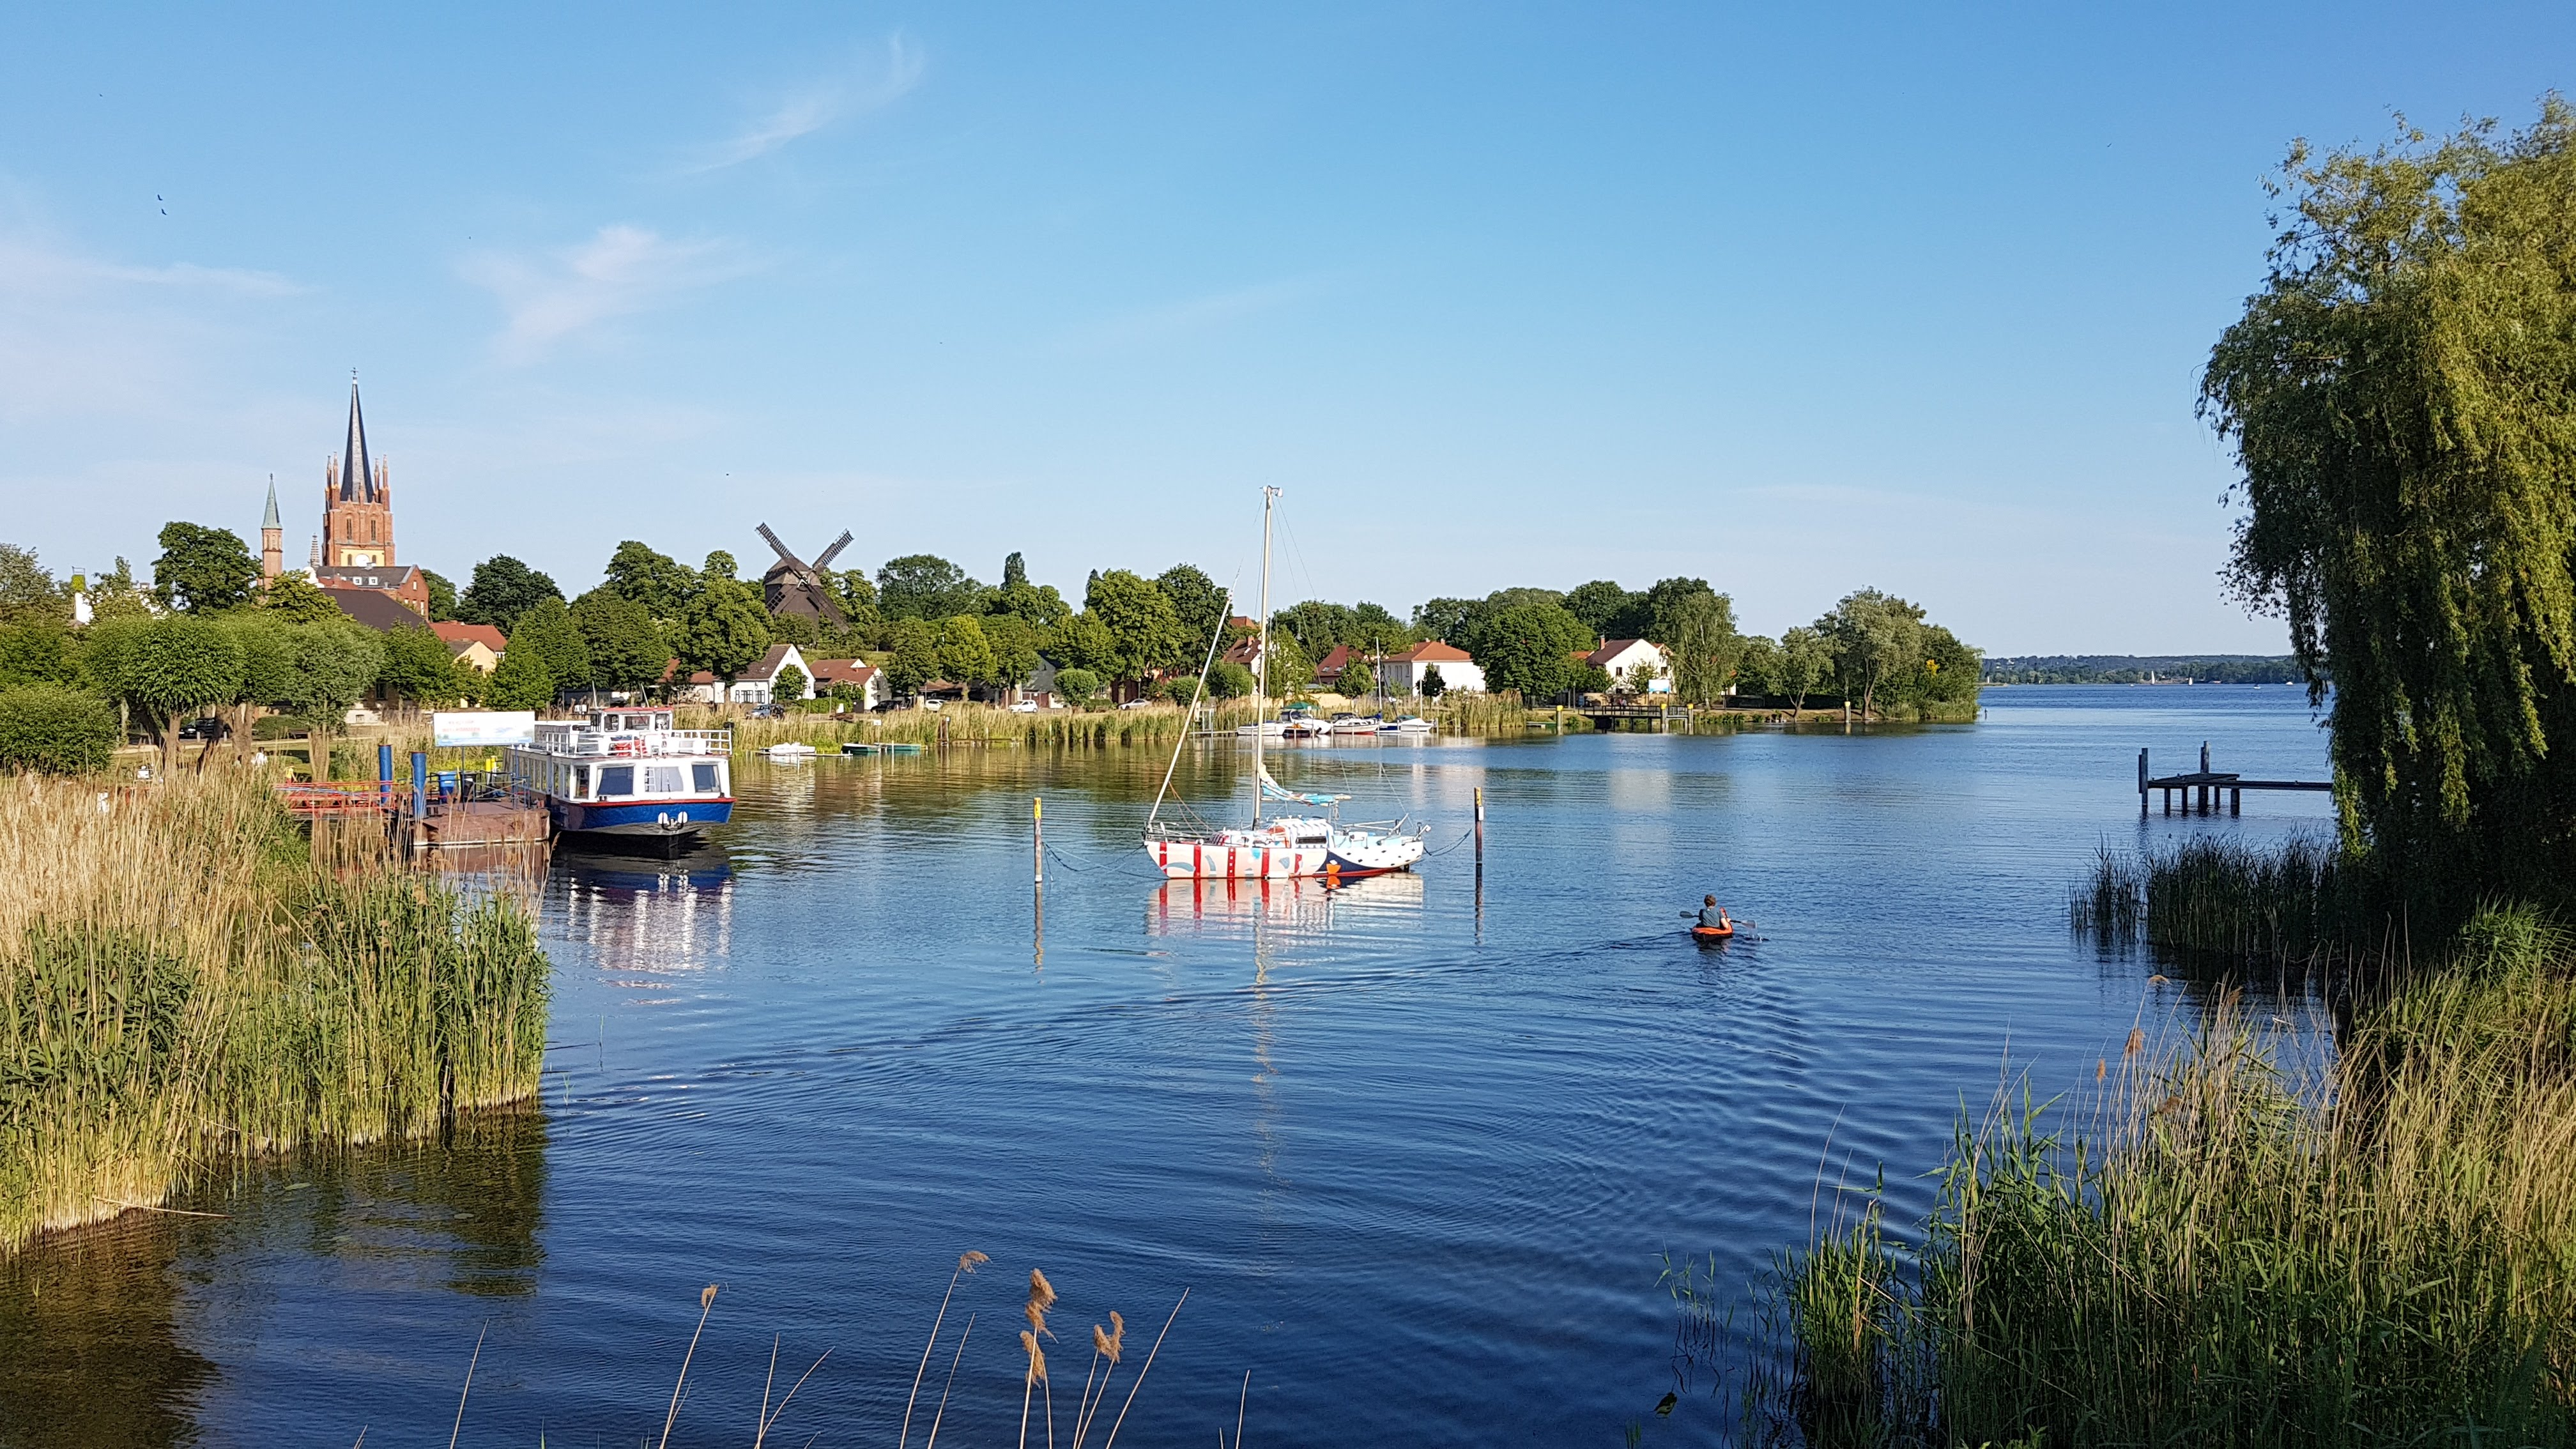
\includegraphics[width=.95\linewidth]{graph/werder.jpg}
	\end{figure}
	\end{minipage}%
	\begin{minipage}{0.3\textwidth}
	\centering
		\begin{figure}
		\centering
		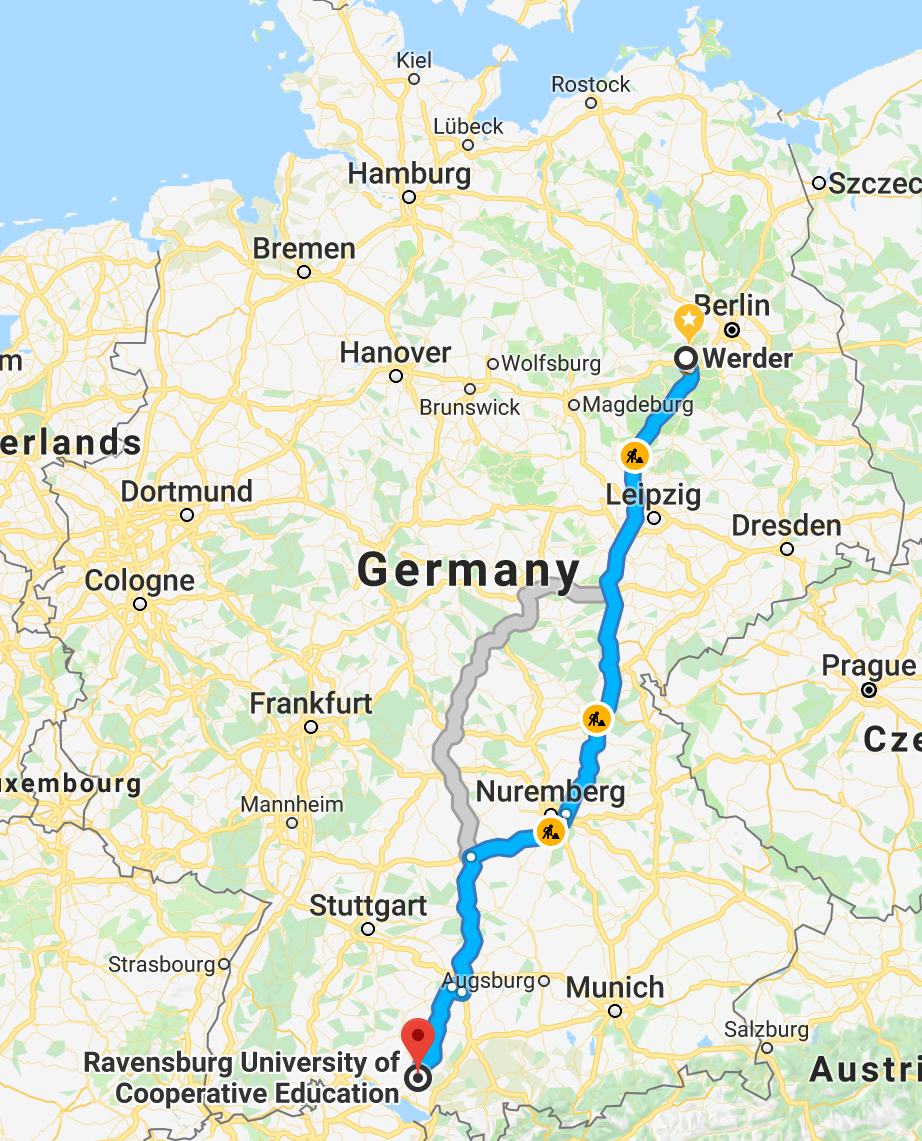
\includegraphics[width=.95\linewidth]{graph/route2werder.png}
		\end{figure}
	\end{minipage}
	\\
	\tiny{Bildquelle: \cite{pic:werder}}
\end{frame}

\begin{frame}{Beruflicher\&Akademischer Werdegang}{}
	\begin{itemize}
		\item \textbf{Juli 2015} - Abitur
		\item \textbf{Ab September 2015} - Duales Studium
		\begin{itemize}
			\item Hochschule: DHBW Ravensburg \textbf{Campus Friedrichshafen}
			\item Studiengang: Informationstechnik (Mobile Informatik)
			\item Firma: Airbus Defence and Space (Immenstaad)
		\end{itemize}
		\item \textbf{September 2018} - Bachelorarbeit und -abschluss
		\item \textbf{Seit Oktober 2018} - Software Architect bei Airbus
	\end{itemize}
\end{frame}
	
\begin{frame}{Was habe ich bisher gemacht?}{Praxisphasen}
		\begin{itemize}
			\item Arbeit im Bereich SIGINT(Signal Intelligence)
			\item Implementierung des TCP Stacks zur Übertragung von Signaldaten(C++, Matlab, Simulink)
			\item Später Abteilungswechsel zu Simulationssoftware
			\item Implementierung eines neuen Schadenmodells in das bestehende System (C++)
			\item \textbf{Analyse und Bewertung neuer Methoden zur Durchführung simulationsgestützter Parameterstudien mit cloud-basierten Systemen} (Bachelorarbeitsthema)
		\end{itemize}
\end{frame}
	
\begin{frame}{Was habe ich bisher gemacht?}{Theoriephasen}
	\begin{itemize}[<+->]
		\item Mathetutorium für untere Semester
		\item Studienarbeit: Entwickeln eines selbstlernenden Chatbots (Tensorflow, Python)
		\begin{itemize}
			\item Mit fraglichen Erfolgen
		\end{itemize}
		\item Dreimaliger Teilnehmer des Bierathlons Friedrichshafen
		\begin{itemize}
			\item 3. Platz
		\end{itemize}
		\item Organisator des alljährlichen Glühweingrillens Friedrichshafen (Nächster Termin: 27. April 2019)
	\end{itemize}
\end{frame}
	
\begin{frame}{Was habe ich bisher gemacht?}{Studienarbeit}
	\begin{alertblock}{Olaf's erste Worte}
	\huge\textbf{"`they're just fucking fucking fucking not just fucking with"'}\par
	\end{alertblock}
\end{frame}